%=====
%===== SECTION "Architecture du projet" =====
%=====
\section{Processus global de surveillance des individus}\label{Methodes}


Le processus  de surveillance des patients est inspiré globalement des méthodes de \textit{concept drift} qui permettent de capturer l'apparition de nouveaux concepts au cours du temps. Nous avons repris l'architecture de \cite{Gama2014} que nous avons modifié pour intégrer le fait que nous ne connaissons pas la véritable nature des données (niveau de risque à prédire) sans intervention du professionnel de santé et pour intégrer des règles expertes pour la levée d'alerte. 

Le processus est organisé  en  $3$ modules indépendants décrit comme suit :
1) la mémorisation et le prétraitement des messages (voir Section \ref{module1});
2) la détection du niveau de risque associé à un message (voir Section \ref{module2});
3) la levée d'alerte (voir Section \ref{module3}).

Les deux premiers modules font une analyse individuelle des messages, le troisième récupère alors les messages d'un même utilisateur afin de les comparer pour lever ou non une alerte.

%*** SUBSECTION "Module de mémorisation des données" ***
\subsection{Module 1 : mémorisation des messages et prétraitements}\label{module1}

L'objectif de ce module est de mémoriser pour chaque personne monitorée :
%La mémorisation des messages est nécessaire car lors de la classification d'un message, les anciens messages du même auteur peuvent avoir de l'importance. Ainsi, lors de la réception d'un nouveau message, il faut être capable de déterminer le niveau de risque des anciens messages.
%Lors de la mémorisation des exemples, le module mémorise toutes les informations liées à l'exemple :
\begin{itemize}
\item le groupe Facebook auquel elle appartient ainsi que la thématique du groupe (e.g. tentative de suicide, harcèlement, anorexie, etc);
\item le contenu de ses messages,  la date et l'heure de l'écriture des messages, le nombre de mentions \emph{likes}, le nombre de commentaires;
\item les commentaires associés à un message;
\end{itemize}

Il est important de noter que cette démarche est aussi applicable à de nombreux autres réseaux sociaux (e.g Twitter, Instagram, Ask... ).

Comme indiqué par \cite{Balahur2013}, les textes issus des réseaux sociaux ont des particularités linguistiques qui peuvent influencer les performances de la classification. Pour cette raison nous avons appliqué les prétraitements suivants :
1) remplacement des noms d'utilisateurs par [NOM];
2) remplacement des adresses mails par [MAIL];
3) remplacement des adresses URL par [URL];
4) remplacement des émoticônes par un mot d'humeur associé (table de correspondance créée pour l'étude);
5) remplacement des abréviations par le(s) mot(s) complet(s) (table de correspondance créée pour l'étude);
6) suppression des accents et des majuscules, en effet certaines personnes n'utilisent pas ces deux conventions d'écritures sur les réseaux sociaux afin d'écrire plus vite. Leur normalisation en minuscules sans accent permet alors de restreindre le nombre de N-Grammes générés et ainsi faire le lien entre des messages ne présentant par avant aucun N-Grammes;
7) lemmatisation de tous les mots en utilisant l’outil TreeTagger (\cite{Schmid1994}).
%*** SUBSECTION "Module d'apprentissage" ***
\subsection{Module 2 : détection du niveau de risque en 2 étapes}\label{module2}

Le module de détection du niveau de risque se déroule en 2 étapes.
Nous avons choisi de travailler en respectant le paradigme de l’ensemble learning qui consiste à apprendre plusieurs classifieurs dans le but de résoudre le même problème.
%Les premiers travaux consacrés à l’ensemble learning datent des années 1990  (\textbf{\cite{Hancock1990, Wolpert1992, Krogh1995, Aze2012}}). Par opposition à l’apprentissage “classique” où un seul classifieur est appris, l’ensemble learning apprend un ensemble de classifieurs qui sont ensuite combinés pour obtenir un méta-classifieur. 

Nous nous sommes placés dans ce paradigme pour les quatre raisons suivantes : 1) la combinaison de classifieurs donne en général de meilleurs résultats (\cite{wang2003mining}); 2) la puissance de calcul à notre disposition rend accessible l’apprentissage et l’utilisation de nombreux modèles pour résoudre le même problème ; 3) les  masses de données à traiter  pourraient s’avèrer  non apprenables par un unique classifieur;
4) le besoin d'expliciter les résultats de la classification pour les humains impliqués dans le processus de prise de décision. %Nous reviendrons sur ces trois éléments lors de l'évaluation de notre méthode.

Diverses formes d’ensemble learning peuvent être citées : \emph{Stacking}, \emph{Boosting} et \emph{Bagging}. 
%Elles divergent principalement par la fonction d’aggrégation mise en œuvre pour obtenir le méta-classifieur. Ces divergences peuvent avoir un impact sur l’apprentissage : modification des exemples pendant l’apprentissage (Stacking), modification de l’importance relative des exemples (Boosting); ou uniquement en post-traitement de l’apprentissage pour combiner les différents modèles appris (Bagging).
Dans notre contexte, nous avons choisi l'approche \emph{Stacking} qui consiste à apprendre une succession de classifieurs organisés en  deux niveaux et aggrégés selon un vote majoritaire et tels que chaque classifieur apprenne de nouveaux descripteurs permettant de redécrire les données.

Nous détaillons dans la suite ces deux étapes dans les sections  \ref{etape1} et  \ref{etape2}.

\subsubsection{Première étape : détection des concepts dans un message}\label{etape1}

La première étape permet de repérer dans les messages un premier niveau d'information :   la présence ou l'absence d'un signal de mal-être que nous nommerons par la suite \emph{concept}. La liste des \emph{concepts} considérés est: \emph{précédente tentative de suicide}, \emph{idéations suicidaires}, \emph{dépression}, \emph{harcèlement}, \emph{prise aux médicaments}, \emph{problème d'alimentation} (anorexie ou boulimie), \emph{auto-mutilation}, \emph{colère}, \emph{peur}, \emph{solitude}, \emph{tristesse} et  \emph{rémission}. Cette liste issue des travaux de \cite{Plutchik1994} a été validée par des experts psychiatres. Pour chaque concept, un classifieur renvoie la valeur \emph{oui} ou \emph{non} pour associer la présence ou l'absence du concept dans le message. 
Nous avons choisi  les descripteurs résumés ci-dessous que nous avons complétés avec des lexiques spécifiques pour chaque concept. 

%\section{Caractéristiques utilisées} \label{caracteristiques}
%*** SUBSECTION "Caractéristiques provenant de Facebook" ***
%\subsection{Caractéristiques provenant de Facebook}
%Plusieurs informations pouvant déterminer le niveau de risque d'un exemple proviennent directement de Facebook. Leur prise en compte est donc indispensables à une bonne classification : 
\begin{itemize}

\item Contenu du message décrit par les mesures statistiques suivantes : 1) un ensemble de N-grammes pour permettre une comparaison entre les messages sélectionnés selon la mesure \emph{TF-IDF} pour ne conserver que les mots discriminants par concepts ; % \textbf{Moins qu'à son habitude}\\ 
%2)  la présence d'élément subjectifs dans la phrase : nous avons réutilisé la chaîne de traitements produite dans l'équipe \cite{Abdaoui2015} qui classe les phrases dans les catégories \textit{information}  (e.g. partage d'un lien relatant une histoire de harcèlement) ou \textit{subjective} (e.g.  confidence de la victime sur un harcèlement subit plus tôt dans la journée);
%3) le nombre de mots de polarité(s) (\textit{négatif, positif ou neutre}) et d'émotion(s) (\textit{joie, colère, etc.}) : l'apparition des sentiments dans les récits est fréquent voir omni-présente. La \emph{peur} est le sentiment le plus  souvent rencontré avec la \emph{tristesse} et la \emph{colère} (voir annexe \ref{annexe_sentiments}). Nous avons utilisé le lexique \cite{Abdaoui2014} produit dans l'équipe et décrit dans l'annexe \ref{annexe_feel} ; 
%\item    Polarité des commentaires d'un exemple & Pour compléter l'orientation d'un message, la mesure définissant la polarité majoritaire des commentaires est définie. La polarité peut est positive, négative ou neutre. Pour cela, on utilise un module externe réalisé au sein de l'équipe [REF]\textbf{Ref Amine et Mike}.\\
 %La notion d'estimation du niveau de risque ne porte que sur le second cas car seul ce type de message décrit l'état de la victime. Il est donc intéressant de pouvoir repérer les messages n'apportant qu'une information.
2) le nombre de mots associés à un concept donné par un lexique réalisé pour l'étude.
\item Nombre de commentaires : un message à risque est suceptible de soulever beaucoup de réactions auprès des autres membres du groupe ;
\item Nombre de mentions \emph{Likes} : à l'inverse, un message où la victime évoque son bien-être ou son rétablissement peut être accompagné de beaucoup de mentions \emph{Likes} ;
\item Longueur du message : deux comportements opposés des victimes sont connus \textcolor{red}{REF}. La victime peut écrire des messages plus longs par besoin de se confier aux autres ou au contraire se refermer sur elle-même et moins écrire;

%\item    Niveau de risque des messages précédents : %le passé de la victime est important  car une personne étant déjà passée à l'acte est plus susceptible de recommencer.  
%Si les exemples précédents ont un haut niveau de risque, un risque de passage à l'acte est plus plausible. Pour calculer la valeur de cette caractéristique, la moyenne du niveau des anciens messages est calculé mais d'autres approches pourraient être testées (e.g. nombre de messages de chaque niveau).
\end{itemize}



En sortie de cette étape, un message est associé à un vecteur de concepts dans lesquels on stocke un booléen.
Par exemple, le message "\textit{Je vais tres mal, aidez moi vite svp. Je me fais harcelee depuis 3ans et me fais frapper tous les jours. Je mappelle lea, jai 14ans et vis a roubaix}" est associé au vecteur 
(
$\overline{\mbox{\emph{tentative de suicide}}}$, 
$\overline{\mbox{\emph{idéations suicidaires}}}$,
$\overline{\mbox{\emph{dépression}}}$,
\emph{harcèlement},
$\overline{\mbox{\emph{médicaments}}}$,
$\overline{\mbox{\emph{anorexie}}}$,
$\overline{\mbox{\emph{mutilation}}}$,
$\overline{\mbox{\emph{colère}}}$,
\emph{peur},
$\overline{\mbox{\emph{solitude}}}$,
\emph{tristesse},
$\overline{\mbox{\emph{rémission}}}$
).

%\paragraph{Présence d'un élément complémentaire au message (lien, photo, etc. )} : Certaines personnes postent une photo pour accompagner 


%*** SUBSECTION "Caractéristiques calculés" ***
%\subsection{Caractéristiques calculées} 
%Afin de compléter la liste des caractéristiques définissant un exemple, d'autres caractéristiques sont calculées en se basant sur les caractéristiques précédemment citées.


\subsubsection{Deuxième étape : calcul du niveau de risque pour un message}\label{etape2}

La seconde étape utilise les sorties de la première étape comme descripteurs pour prédire le niveau de risque des messages. Les niveaux de risque sont répartis sur cinq niveaux représentant les messages non à risque (niveau 0), présentant un ancien risque (niveau 1), à risque faible (niveau 2), à risque modéré (niveau 3), à risque élevé (niveau 4).

Les $5$ niveaux de risque en sortie étant difficiles à interpréter en terme de levée d'alerte, nous avons simplifié le problème en prédisant $2$ niveaux de risque après regroupement des niveaux 0 et en \textit{risque faible} ainsi que 2, 3 et 4 en \textit{risque élevé}.
%*** SUBSECTION "Module d'estimation des pertes" ***
\subsection{Module 3 : levée d'une alerte}\label{module3}

Pour la levée d'une alerte, nous avons décidé de comparer 3 modèles : 1) un modèle de dérive des concepts via l'estimation classique des pertes  en \textit{concept drift} (voir  section  \ref{pertes}); 2) un modèle par comparaison de courbe ROC (voir  section \ref{roc}); 3)  un modèle basé sur des règles expertes telles que fournies par l'association partenaire (voir  section  \ref{regles}).

\subsubsection{Modèle basé sur l'estimation des pertes}\label{pertes}

La plupart des algorithmes de \emph{concept drift} \cite{Gama2014} considèrent des tâches pour lesquelles on connait, à un certain moment, la vraie valeur associée aux données à prédire. Par exemple, pour des relevés de températures, on peut prédire des valeurs puis mesurer la vraie valeur que l'on peut comparer aux prévisions pour estimer les pertes, c'est-à-dire l'écart entre la prédiction et la vérité et lever une alerte si les pertes sont trop élevées (i.e les prédictions sont trop souvent fausses). Dans notre cas, la "vérité" n'est pas disponible sans intervention du professionnel de santé que l'on souhaite minimiser. Nous avons donc adapté le calcul réalisé par \cite{Bach2010} pour estimer les pertes à un instant donné en considérant le taux d'accord entre les classifieurs (i.e on compte le nombre de classifieurs ayant réalisé la même prédiction).

Soit une fenêtre $\mathcal{F}$ glissante contenant les $N$ derniers exemples de l'utilisateur (lors de l'arrivée d'un nouveau message, le plus ancien est supprimé). Le $1^{er}$ et le $N^e$ exemples décrivent respectivement le message le plus ancien et le plus récent.
Le taux d'erreur $\delta$ au temps $t$, noté $\delta_t$ est donné par :
\[
\delta_t = \frac{\sum\limits_{i=1}^N bienClasse(i)}{N}
\]

où $bienClasse(i)$ retourne le taux d'accord de la prédiction retenue (i.e le nombre de classifieurs ayant prédit le niveau retenu sur le nombre de classifieurs). 

Cependant, il est important de pondérer l'instant dans le temps d'une erreur de classement. Pour cela, un système d'\emph{oubli progressif} (\cite{Chandramouli}) est mis en place. Ainsi, chaque erreur est coefficientée selon son ancienneté :
\[
\delta_t = \frac{\sum\limits_{i=1}^N (bienClasse(i)*\frac{i}{N})}{\frac{N+1}{2}}
\]

Les $N$ dernières valeurs $\delta$ sont mémorisées, soit le $\delta$ associé à chacun des $N$ messages précédemment nommés. 
Une alerte est levée si la moyenne des $N$ $\delta$ dépasse un seuil $\Delta$ fixé par l'utilisateur. Si c'est le cas, l'ensemble des $N$ valeurs $\delta$ sont transmises au module de détection de changement pour calculer le temps pour lequel le changement a eu lieu et lancer une procédure d'alerte auprès du psychiatre référent. 

Pour l'interprétation du professionnel de santé, il est important de lui pointer le temps où un concept est apparu pour l'aider dans son analyse.
Si une dérive du modèle est constatée, il faut réapprendre un nouveau modèle à partir de ce moment. Pour cela, on cherche $\Omega$ tel que :
\begin{itemize} 
\item $\Omega$ soit l'indice de l'exemple parmi l'ensemble des $N$ exemples. Soit $1 \leq \Omega \leq N$;
\item La différence des moyennes des valeurs d'estimation des pertes des sous-ensembles définit par les bornes $[1,\Omega-1]$ et $[\Omega,N]$ soit maximale.
\end{itemize}

Ainsi, l'algorithme~\ref{algo:cd}, que nous proposons, donne le temps $t$ où le changement de concept est le plus plausible. Afin de déterminer au mieux l'instant du changement de comportement.

\begin{algorithm}
\DontPrintSemicolon
\Donnees{Une fenêtre glissante $\mathcal{F}=\{\delta_1, \delta_2, \ldots, \delta_N\}$ de valeurs numériques}
\Res{L'indice $\Omega$ qui maximise l'écart de moyenne entre les sous-ensembles $\mathcal{F}_1$ et $\mathcal{F}_2$ bornés respectivement par $[1,\Omega-1]$ et $[\Omega,N]$}
$\Omega \gets 1$\;
$diff_\Omega \gets 0$\;
\Pour{$i \gets 2$ \textbf{à} $N$} {
	$somme_1 \gets 0$\;
	\Pour{$j \gets 1$ \textbf{à} $i-1$} {
    	$somme_1 = somme_1+ \mathcal{F}_{j}$\;
    }
    $moyenne_1 \gets \frac{somme_1}{i-1}$\;
    
    $somme_2 \gets 0$\;
	\Pour{$j \gets i$ \textbf{à} $N$} {
    	$somme_2 = somme_2+ \mathcal{F}_{j}$\;
    }
    $moyenne_2 \gets \frac{somme_2}{(N-i)+1}$\;
  \Si{$diff_\Omega < |moyenne_1-moyenne_2|$} {
    $\Omega = i$\;
    $diff_\Omega = |moyenne_1-moyenne_2|$\;
  }
}
\Retour{$\Omega$}\;
\caption{{\bsc{Detection du temps de Changement}}}
\label{algo:cd}
\end{algorithm}
\subsubsection{Modèle basé sur la comparaison de courbe ROC}\label{roc}

% Nous avons ici reformuler le problème pour lever une alerte quand on trouve au moins un message posté par l'utilisateur  tel que le niveau de risque associé à ce message soit élevé. Pour atteindre cet objectif, plusieurs approches peuvent être mise en \oe uvre : apprentissage de classifieurs pour le niveau de risque (classification), apprentissage d'une fonction permettant d'associer un risque à chaque message (régression) ou encore apprentissage d'une fonction permettant d'ordonner les messages par risque croissant.

% L'approche que nous allons présenter ici relève de ce dernier cas d'utilisation.
% Nous allons utiliser l'algorithme ROGER (ROc based Genetic learnER) initialement proposé en 2003 dans le cadre de la prédiction du risque cardio-vasculaire \cite{SebagAzeLucas:ICDM2003,SebagLucasAze:EA2003,Challenge_PKDD03}.
% Cet algorithme a été adapté et utilisé avec succès dans plusieurs autres cadres applicatifs : l'extraction de la terminologie \cite{Aze_ROCML:2005}, de la prédiction d'interactions entre protéines \cite{deVienne-Aze_PLoSOne:2012} ou encore de la prédiction de complexes protéines-protéines \cite{PLoSOne:2011}.

% L'algorithme ROGER apprend des fonctions de la forme : $f({\bm x_i}) = \sum_j w_j \times {\bm x_i}(j)$ où ${\bm x_i}(j)$ représente la valeur de la  $j^{ème}$ composante de l'exemple ${\bm x_i}$.
% L'algorithme apprend les poids $w_j$ tels que $\sum_i rang_f({\bm x_i}) \times \mathds{1}_{y_i = +1}$ soit minimale (où $rang_f({\bm x_i})$ correspond au rang de l'exemple ${\bm x_i}$ induit par la fonction $f$, et $\mathds{1}_{y_i = +1}$ correspondant à la fonction indicatrice qui vaut 1 si la classe de ${\bm x_i}$ est positive et 0 sinon).

% Il est aisé de montrer qu'une fonction maximisant l'aire sous la courbe ROC minimise la somme des rangs des exemples positifs qu'elle ordonne.

La  \textbf{courbe ROC} (Receiver Operating Characteristic) \cite{RocLift:2006,ROC:1978} représente un classifieur ayant la capacité de séparer parfaitement les positifs des négatifs.

Nous allons utiliser l'algorithme ROGER (ROc based Genetic learnER) initialement proposé en 2003 dans le cadre de la prédiction du risque cardio-vasculaire \cite{SebagAzeLucas:ICDM2003,SebagLucasAze:EA2003,Challenge_PKDD03}. Cet algorithme a été adapté et utilisé avec succès dans plusieurs autres cadres applicatifs : l'extraction de la terminologie \cite{Aze_ROCML:2005}, de la prédiction d'interactions entre protéines \cite{deVienne-Aze_PLoSOne:2012} ou encore de la prédiction de complexes protéines-protéines \cite{PLoSOne:2011}.

L'algorithme ROGER apprend des fonctions de la forme : $f({\bm x_i}) = \sum_j w_j \times {\bm x_i}(j)$ où ${\bm x_i}(j)$ représente la valeur de la  $j^{ème}$ composante de l'exemple ${\bm x_i}$.
L'algorithme apprend les poids $w_j$ tels que $\sum_i rang_f({\bm x_i}) \times \mathds{1}_{y_i = +1}$ soit minimale (où $rang_f({\bm x_i})$ correspond au rang de l'exemple ${\bm x_i}$ induit par la fonction $f$, et $\mathds{1}_{y_i = +1}$ correspondant à la fonction indicatrice qui vaut 1 si la classe de ${\bm x_i}$ est positive et 0 sinon).


Dans notre contexte, ROGER permet d'apprendre à ordonner les messages des utilisateurs par risque décroissant.
Sous l'hypothèse qu'il existe au moins un \textit{concept drift} par utilisateur, nous considérons que le message le plus à risque (prédit par ROGER) est le message correspondant au drift.
\subsubsection{Modèle basé sur les règles expertes}\label{regles}

%La troisième couche consiste à classer l'instance en deux classes (\textit{alerte} et \textit{non alerte}) selon des règles expertes.  
%Comme il n'est pas possible de compter en permanence sur la participation du professionnel pour étiquer les messages et calculer l'estimation des pertes, 
Nous avons également implémenté des règles expertes fournies par l'association \textit{OADI} pour la levée de l'alerte et nous avons exploré les scénarios suivants. Une alerte est levée si il y a : 
1) un message avec un risque  de niveau 4 dans les $N$ derniers messages;
2)  une augmentation du niveau de risque entre 2 temps consécutifs;
3)  une augmentation du niveau de risque avec un écart de au moins 2 niveaux sur une fenêtre de $N$ messages; Nous ferons varier $N$ pour évaluer les performances pour détecter des changements abrupts ou lents;
4)  des oscillations du niveau de risque.

On obtient alors les règles suivantes : Soit $M$ l'ensemble des $N$ derniers messages d'un utilisateur où $M_1$ correspond au message le plus ancien et $M_N$ au plus récent. On notera $R_i$ le niveau de risque du message $i$.

% * <jeromeaze@gmail.com> 2015-09-21T10:03:18.541Z:
%
%  Dans le contexte, je ne comprend pas 
%
\begin{itemize}
\item  $\exists i, 0\leq i \leq N | R_i = 4$
\item  $\exists i, 0\leq i \leq N-1 | R_i < R_{i+1}$
\item  $\exists i, 0\leq i \leq N-1 | R_i < (R_{i+1}-1)$
\item  $\exists i \exists j, 0\leq i \leq N-1, 0\leq j \leq N-1 | R_i < R_{i+1}, R_j > (R_{j+1})$
\end{itemize}

\begin{figure}[!h]
   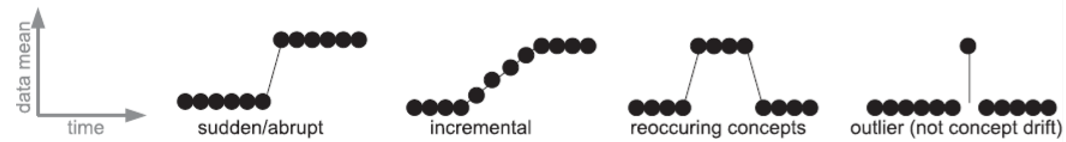
\includegraphics[width=.95\textwidth]{imgs/types_concept_drift.png}
	\caption{\label{formes_cd} Les différentes formes de \emph{concept drift} (adaptés de \cite{Gama2014})}
\end{figure}

Le schéma \ref{formes_cd} représente les différentes formes de changement que nous souhaitons capturer via les règles expertes : 
1) Le changement \emph{immédiat} correspond à un individu qui parle du jour au lendemain de méthode de suicide;
2) Le changement \emph{incrémental} correspond au cas où l'individu parle de plus en plus de son mal être;
3) Le changement \emph{récurrent} est un utilisateur qui régulièrement parle de son mal être;
4) Le \emph{bruit} serait un message isolé parlant de suicide.

%En sortie de ce module, quelque soit les variantes implémentées, nous obtenons la levée ou non d'une alerte pour un individus, le message ayant sucité la levée de l'alerte, les annotations en terme de concept et de risque (issue du module 2) qui vont aider le professionnel de santé à prendre la décision d'intervenir ou non.